\documentclass[a4paper,11pt]{article}
\usepackage[utf8]{inputenc}
\usepackage[T1]{fontenc}
\usepackage{amsmath,amssymb}
\usepackage[a4paper,left=2cm,right=2cm,top=3.6cm,bottom=2.3cm,headheight=1.1cm,headsep=0.6cm,footskip=1cm]{geometry}
\usepackage{xcolor}
\usepackage{tikz}
\usetikzlibrary{calc,arrows.meta}
\usepackage{fancyhdr}
\usepackage{lastpage}
\usepackage{tabularx}
\usepackage{array}
\usepackage[most]{tcolorbox}
\usepackage{enumitem}
\usepackage{needspace}

\definecolor{navy}{HTML}{1F3A5F}
\definecolor{teal}{HTML}{0F8B7D}
\definecolor{softbg}{HTML}{F4F7FA}
\definecolor{brick}{HTML}{B03A2E}
\newcommand{\dis}{\displaystyle}

\setlength{\parindent}{0pt}
\renewcommand{\arraystretch}{1.35}

% ---------- header berwarna navy ----------
\pagestyle{fancy}
\fancyhf{}
\renewcommand{\headrulewidth}{0pt}
\fancyhead[L]{%
  \begin{tikzpicture}[remember picture,overlay]
    \fill[navy] ([yshift=-1.2cm]current page.north west) rectangle ([yshift=-3.15cm]current page.north east);
    \fill[teal] ([yshift=-3.15cm]current page.north west) rectangle ([yshift=-3.25cm]current page.north east);
  \end{tikzpicture}%
  \color{white}\bfseries\large Latihan Soal Perbandingan Trigonometri}
\fancyhead[R]{\color{white}\small Diunduh dari website \textbf{Math1729}\ \,|\,\ 4 Oktober 2026}
\fancyfoot[L]{\small\color{navy}Math1729 --- Perbandingan Trigonometri}
\fancyfoot[R]{\small\color{navy}Halaman \thepage\ dari \pageref{LastPage}}

% ---------- komponen ----------
\newcounter{no}
\newcommand{\bagian}[2]{\par\Needspace{6\baselineskip}\vspace{1.0em}\noindent
  \begin{tcolorbox}[colback=navy,colframe=navy,coltext=white,boxrule=0pt,arc=2pt,left=6pt,right=6pt,top=3pt,bottom=3pt]
  \textbf{#1}\hfill{\small #2}\end{tcolorbox}\setcounter{no}{0}\par\vspace{-0.3em}}
\newcommand{\tingkat}[2]{\par\Needspace{7\baselineskip}\vspace{0.6em}\noindent
  {\color{teal}\rule{3pt}{1.1em}}\ {\color{navy}\bfseries #1}\ {\small\color{gray}--- #2}\par\vspace{0.1em}}
\newcommand{\soal}[2]{\par\vspace{0.75em}\stepcounter{no}\noindent
  \begin{minipage}[t]{1.8em}\textbf{\theno.}\end{minipage}%
  \begin{minipage}[t]{\dimexpr\linewidth-1.8em\relax}#1\par\vspace{0.35em}#2\end{minipage}\par}
\newcommand{\poin}[1]{\hfill{\small\color{navy}[#1 poin]}}

% teks di kiri, gambar di kanan
\newcommand{\gbr}[2]{\noindent\begin{minipage}[t]{0.58\linewidth}#1\end{minipage}\hfill\raisebox{\ht\strutbox}{\begin{minipage}[t]{0.39\linewidth}\vspace{0pt}\centering#2\end{minipage}}}
% tanda sudut siku-siku di titik #2 (antara #1 dan #3); dipakai di dalam tikzpicture
\newcommand{\siku}[3]{\coordinate (sk1) at ($(#2)!0.2cm!(#1)$); \coordinate (sk2) at ($(#2)!0.2cm!(#3)$);
  \draw[navy,thin] (sk1) -- ($(sk1)+(sk2)-(#2)$) -- (sk2);}
\tikzset{tri/.style={thick,navy,fill=softbg}}

\begin{document}
\thispagestyle{fancy}

\begin{center}
  {\color{navy}\fontsize{22}{26}\selectfont\bfseries Latihan Soal Perbandingan Trigonometri\par}
\end{center}
\vspace{2pt}
\begin{tcolorbox}[colback=softbg,colframe=navy!40,boxrule=0.6pt,arc=3pt,left=8pt,right=8pt,top=5pt,bottom=5pt]
\noindent\textbf{Nama} : \rule{4.6cm}{0.4pt}\hfill\textbf{Kelas} : \rule{2.2cm}{0.4pt}\hfill\textbf{Skor} : \rule{2.2cm}{0.4pt}
\end{tcolorbox}
\vspace{2pt}
\begin{tcolorbox}[colback=white,colframe=teal,boxrule=0.8pt,arc=3pt,left=8pt,right=8pt,top=4pt,bottom=4pt,title={\bfseries Petunjuk Pengerjaan},coltitle=white,fonttitle=\small]
\small
\begin{enumerate}[leftmargin=1.4em,itemsep=1pt,topsep=1pt]
\item Soal terdiri atas \textbf{15 pilihan ganda} (5 mudah, 5 sedang, 5 sulit), \textbf{5 isian singkat}, dan \textbf{3 uraian (essay)}. Alokasi waktu yang disarankan: 90 menit.
\item Skor: pilihan ganda 3 poin, isian singkat 5 poin, uraian 10 poin per soal (total 100 poin). Tidak ada pengurangan skor untuk jawaban salah.
\item Sudut $\theta$ pada soal adalah sudut lancip, kecuali dinyatakan lain. Gambar tidak selalu digambar sesuai skala.
\item Kebalikan: $\csc\theta=\dis\frac{1}{\sin\theta}$, $\sec\theta=\dis\frac{1}{\cos\theta}$, $\cot\theta=\dis\frac{1}{\tan\theta}$. Sudut elevasi adalah sudut antara garis pandang ke atas dan garis mendatar; sudut depresi adalah sudut antara garis pandang ke bawah dan garis mendatar.
\item Kalkulator tidak diperkenankan.
\end{enumerate}
\end{tcolorbox}

\bagian{A. Pilihan Ganda}{15 soal $\times$ 3 poin = 45 poin. Pilih satu jawaban yang paling tepat.}

\tingkat{Tingkat Mudah}{soal 1 sampai 5}
\soal{\gbr{Perhatikan segitiga $PQR$ yang siku-siku di $Q$ pada gambar. Nilai $\cos P$ adalah \dots.}{%
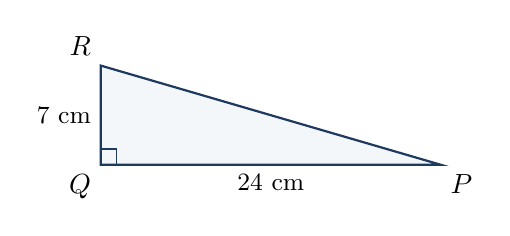
\begin{tikzpicture}
\coordinate (Q) at (0,0); \coordinate (P) at (4.32,0); \coordinate (R) at (0,1.26);
\draw[tri] (P)--(Q)--(R)--cycle;
\siku{P}{Q}{R}
\node[below left] at (Q) {$Q$}; \node[below right] at (P) {$P$}; \node[above left] at (R) {$R$};
\node[below,font=\small] at (2.16,0) {$24$ cm}; \node[left,font=\small] at (0,0.63) {$7$ cm};
\end{tikzpicture}}}{\begin{tabularx}{\linewidth}{@{}*{5}{X}@{}}\textbf{A.}\;$\dis\frac{7}{25}$ & \textbf{B.}\;$\dis\frac{7}{24}$ & \textbf{C.}\;$\dis\frac{24}{25}$ & \textbf{D.}\;$\dis\frac{25}{24}$ & \textbf{E.}\;$\dis\frac{25}{7}$\end{tabularx}}
\soal{Nilai dari $\tan60^\circ\cdot\cos30^\circ-\sin30^\circ$ adalah \dots.}{\begin{tabularx}{\linewidth}{@{}*{5}{X}@{}}\textbf{A.}\;$0$ & \textbf{B.}\;$\dis\frac12$ & \textbf{C.}\;$\dis\frac34$ & \textbf{D.}\;$1$ & \textbf{E.}\;$\dis\frac32$\end{tabularx}}
\soal{Jika $\theta$ sudut lancip dan $\cos\theta=\dis\frac{15}{17}$, maka $\tan\theta=$ \dots.}{\begin{tabularx}{\linewidth}{@{}*{5}{X}@{}}\textbf{A.}\;$\dis\frac{8}{15}$ & \textbf{B.}\;$\dis\frac{15}{17}$ & \textbf{C.}\;$\dis\frac{17}{15}$ & \textbf{D.}\;$\dis\frac{15}{8}$ & \textbf{E.}\;$\dis\frac{17}{8}$\end{tabularx}}
\soal{\gbr{Dina (tinggi matanya $1{,}5$ m dari tanah) berdiri $15$ m dari sebuah gedung. Ia melihat puncak gedung dengan sudut elevasi $45^\circ$ seperti pada gambar. Tinggi gedung adalah \dots.}{%
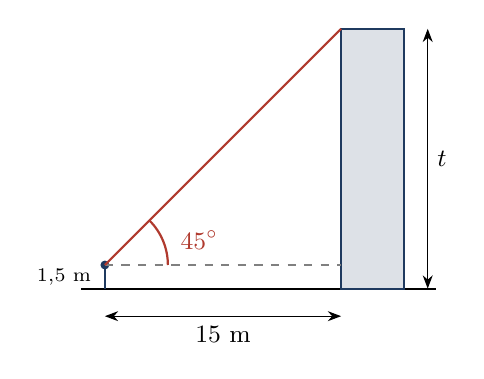
\begin{tikzpicture}
\draw[thick] (-0.3,0)--(4.2,0);
\fill[navy!15,draw=navy,thick] (3,0) rectangle (3.8,3.3);
\draw[thick,navy] (0,0)--(0,0.3); \fill[navy] (0,0.3) circle (1.6pt);
\draw[dashed,gray] (0,0.3)--(3,0.3);
\draw[thick,brick] (0,0.3)--(3,3.3);
\draw[brick,thick] (0.8,0.3) arc (0:45:0.8); \node[brick,font=\small] at (1.2,0.62) {$45^\circ$};
\draw[<->,>=Stealth] (0,-0.35)--(3,-0.35); \node[below,font=\small] at (1.5,-0.35) {$15$ m};
\node[left,font=\scriptsize] at (-0.05,0.15) {$1{,}5$ m};
\draw[<->,>=Stealth] (4.1,0)--(4.1,3.3); \node[right,font=\small] at (4.1,1.65) {$t$};
\end{tikzpicture}}}{\begin{tabularx}{\linewidth}{@{}*{3}{X}@{}}\textbf{A.}\;$15$ m & \textbf{B.}\;$16{,}5$ m & \textbf{C.}\;$15\sqrt2$ m\\[3pt] \textbf{D.}\;$\left(15\sqrt2+1{,}5\right)$ m & \textbf{E.}\;$\left(15\sqrt3+1{,}5\right)$ m & \end{tabularx}}
\soal{Jika $\tan\theta=\dis\frac34$ dengan $\theta$ lancip, maka $\csc\theta=$ \dots.}{\begin{tabularx}{\linewidth}{@{}*{5}{X}@{}}\textbf{A.}\;$\dis\frac35$ & \textbf{B.}\;$\dis\frac45$ & \textbf{C.}\;$\dis\frac54$ & \textbf{D.}\;$\dis\frac43$ & \textbf{E.}\;$\dis\frac53$\end{tabularx}}

\tingkat{Tingkat Sedang}{soal 6 sampai 10}
\soal{\gbr{Pada gambar, segitiga $ABC$ siku-siku di $B$ dengan $AB=6$ cm dan $BC=8$ cm. Titik $D$ terletak pada $AC$ sehingga $BD\perp AC$. Nilai $\cos\angle DBC$ adalah \dots.}{%
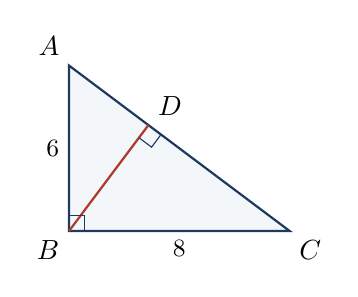
\begin{tikzpicture}
\coordinate (B) at (0,0); \coordinate (A) at (0,2.1); \coordinate (C) at (2.8,0);
\coordinate (D) at ($(A)!(B)!(C)$);
\draw[tri] (A)--(B)--(C)--cycle;
\draw[thick,brick] (B)--(D);
\siku{A}{B}{C}
\siku{B}{D}{C}
\node[above left] at (A) {$A$}; \node[below left] at (B) {$B$}; \node[below right] at (C) {$C$}; \node[above right] at (D) {$D$};
\node[left,font=\small] at (0,1.05) {$6$}; \node[below,font=\small] at (1.4,0) {$8$};
\end{tikzpicture}}}{\begin{tabularx}{\linewidth}{@{}*{5}{X}@{}}\textbf{A.}\;$\dis\frac35$ & \textbf{B.}\;$\dis\frac34$ & \textbf{C.}\;$\dis\frac45$ & \textbf{D.}\;$\dis\frac{24}{25}$ & \textbf{E.}\;$\dis\frac54$\end{tabularx}}
\soal{Nilai dari $\dis\frac{\sin^{2}30^\circ+\cos^{2}45^\circ}{\tan60^\circ\cdot\cot30^\circ}$ adalah \dots.}{\begin{tabularx}{\linewidth}{@{}*{5}{X}@{}}\textbf{A.}\;$\dis\frac1{12}$ & \textbf{B.}\;$\dis\frac14$ & \textbf{C.}\;$\dis\frac13$ & \textbf{D.}\;$\dis\frac12$ & \textbf{E.}\;$\dis\frac34$\end{tabularx}}
\soal{Jika $\theta$ sudut lancip dan $3\sin\theta=2\cos\theta$, maka nilai $\sin\theta\cos\theta$ adalah \dots.}{\begin{tabularx}{\linewidth}{@{}*{5}{X}@{}}\textbf{A.}\;$\dis\frac13$ & \textbf{B.}\;$\dis\frac25$ & \textbf{C.}\;$\dis\frac{6}{13}$ & \textbf{D.}\;$\dis\frac12$ & \textbf{E.}\;$\dis\frac23$\end{tabularx}}
\soal{\gbr{Sebuah tangga sepanjang $8$ m bersandar pada dinding vertikal dan membentuk sudut $60^\circ$ dengan tanah. Kaki tangga ditarik menjauhi dinding sehingga sudutnya menjadi $30^\circ$ (ujung atas tangga tetap menempel di dinding). Ujung atas tangga turun sejauh \dots.}{%
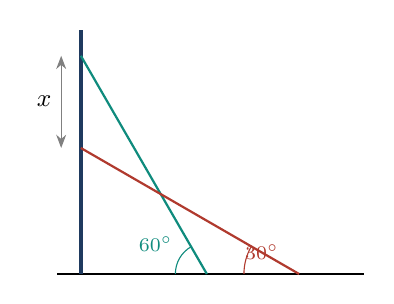
\begin{tikzpicture}
\draw[thick] (-0.3,0)--(3.6,0);
\draw[ultra thick,navy] (0,0)--(0,3.1);
\draw[thick,teal] (1.6,0)--(0,2.771);
\draw[thick,brick] (2.771,0)--(0,1.6);
\draw[teal] (1.2,0) arc (180:120:0.4); \node[teal,font=\scriptsize] at (0.95,0.38) {$60^\circ$};
\draw[brick] (2.071,0) arc (180:150:0.7); \node[brick,font=\scriptsize] at (2.3,0.28) {$30^\circ$};
\draw[<->,>=Stealth,gray] (-0.25,1.6)--(-0.25,2.771); \node[left,font=\small] at (-0.25,2.2) {$x$};
\end{tikzpicture}}}{\begin{tabularx}{\linewidth}{@{}*{3}{X}@{}}\textbf{A.}\;$2\left(\sqrt3-1\right)$ m & \textbf{B.}\;$4\left(\sqrt3-1\right)$ m & \textbf{C.}\;$8\left(\sqrt3-1\right)$ m\\[3pt] \textbf{D.}\;$4\sqrt3$ m & \textbf{E.}\;$4\left(\sqrt3+1\right)$ m & \end{tabularx}}
\soal{\gbr{Segitiga sama kaki $ABC$ dengan $AB=AC=13$ cm dan alas $BC=10$ cm (lihat gambar). Nilai $\sin B+\cos B$ adalah \dots.}{%
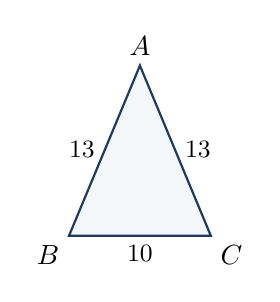
\begin{tikzpicture}
\coordinate (B) at (0,0); \coordinate (C) at (1.8,0); \coordinate (A) at (0.9,2.16);
\draw[tri] (A)--(B)--(C)--cycle;
\node[above] at (A) {$A$}; \node[below left] at (B) {$B$}; \node[below right] at (C) {$C$};
\node[left,font=\small] at (0.45,1.1) {$13$}; \node[right,font=\small] at (1.35,1.1) {$13$}; \node[below,font=\small] at (0.9,0) {$10$};
\end{tikzpicture}}}{\begin{tabularx}{\linewidth}{@{}*{5}{X}@{}}\textbf{A.}\;$\dis\frac5{13}$ & \textbf{B.}\;$\dis\frac{12}{13}$ & \textbf{C.}\;$1$ & \textbf{D.}\;$\dis\frac{17}{13}$ & \textbf{E.}\;$\dis\frac{18}{13}$\end{tabularx}}

\tingkat{Tingkat Sulit}{soal 11 sampai 15, setara UTBK}
\soal{Jika $\theta$ sudut lancip yang memenuhi $\sin\theta+\cos\theta=\dis\frac75$, maka $\tan\theta+\cot\theta=$ \dots.}{\begin{tabularx}{\linewidth}{@{}*{5}{X}@{}}\textbf{A.}\;$\dis\frac{12}{25}$ & \textbf{B.}\;$\dis\frac{7}{12}$ & \textbf{C.}\;$\dis\frac{12}{7}$ & \textbf{D.}\;$\dis\frac{25}{12}$ & \textbf{E.}\;$\dis\frac{49}{12}$\end{tabularx}}
\soal{\gbr{Dari titik $A$ di tanah datar, puncak sebuah menara terlihat dengan sudut elevasi $30^\circ$. Setelah berjalan $20$ m mendekati menara (segaris dengan kaki menara) sampai di titik $B$, sudut elevasinya menjadi $60^\circ$. Tinggi menara adalah \dots.}{%
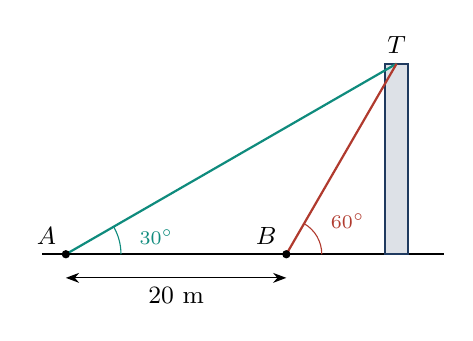
\begin{tikzpicture}
\draw[thick] (-4.5,0)--(0.6,0);
\fill[navy!15,draw=navy,thick] (-0.15,0) rectangle (0.15,2.42);
\draw[thick,teal] (-4.2,0)--(0,2.42); \draw[thick,brick] (-1.4,0)--(0,2.42);
\fill (-4.2,0) circle (1.5pt); \fill (-1.4,0) circle (1.5pt);
\draw[teal] (-3.5,0) arc (0:30:0.7); \node[teal,font=\scriptsize] at (-3.05,0.22) {$30^\circ$};
\draw[brick] (-0.95,0) arc (0:60:0.45); \node[brick,font=\scriptsize] at (-0.62,0.42) {$60^\circ$};
\node[above left,font=\small] at (-4.2,0) {$A$}; \node[above left,font=\small] at (-1.4,0) {$B$};
\draw[<->,>=Stealth] (-4.2,-0.3)--(-1.4,-0.3); \node[below,font=\small] at (-2.8,-0.3) {$20$ m};
\node[above,font=\small] at (0,2.42) {$T$};
\end{tikzpicture}}}{\begin{tabularx}{\linewidth}{@{}*{5}{X}@{}}\textbf{A.}\;$10$ m & \textbf{B.}\;$15$ m & \textbf{C.}\;$10\sqrt3$ m & \textbf{D.}\;$20$ m & \textbf{E.}\;$20\sqrt3$ m\end{tabularx}}
\soal{\gbr{Pada gambar, segitiga $ABC$ siku-siku di $B$ dengan $AB=6$ cm, $\angle BAD=30^\circ$, dan $\angle BAC=60^\circ$ (titik $D$ pada $BC$). Luas segitiga $ACD$ adalah \dots.}{%
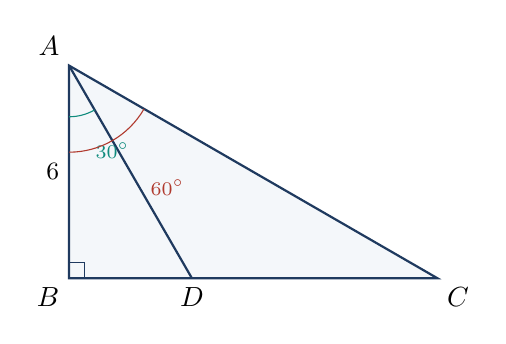
\begin{tikzpicture}
\coordinate (B) at (0,0); \coordinate (A) at (0,2.7); \coordinate (D) at (1.56,0); \coordinate (C) at (4.677,0);
\draw[tri] (A)--(B)--(C)--cycle; \draw[navy,thick] (A)--(D);
\siku{A}{B}{C}
\draw[teal] (0,2.05) arc (-90:-60:0.65); \node[teal,font=\scriptsize] at (0.55,1.62) {$30^\circ$};
\draw[brick] (0,1.6) arc (-90:-30:1.1); \node[brick,font=\scriptsize] at (1.25,1.15) {$60^\circ$};
\node[above left] at (A) {$A$}; \node[below left] at (B) {$B$}; \node[below] at (D) {$D$}; \node[below right] at (C) {$C$};
\node[left,font=\small] at (0,1.35) {$6$};
\end{tikzpicture}}}{\begin{tabularx}{\linewidth}{@{}*{5}{X}@{}}\textbf{A.}\;$6$ cm$^2$ & \textbf{B.}\;$6\sqrt3$ cm$^2$ & \textbf{C.}\;$12$ cm$^2$ & \textbf{D.}\;$18$ cm$^2$ & \textbf{E.}\;$12\sqrt3$ cm$^2$\end{tabularx}}
\soal{Jika $\theta$ sudut lancip dan $\sin\theta-\cos\theta=\dis\frac12$, maka $\sin^{4}\theta+\cos^{4}\theta=$ \dots.}{\begin{tabularx}{\linewidth}{@{}*{5}{X}@{}}\textbf{A.}\;$\dis\frac{23}{32}$ & \textbf{B.}\;$\dis\frac34$ & \textbf{C.}\;$\dis\frac78$ & \textbf{D.}\;$\dis\frac{15}{16}$ & \textbf{E.}\;$1$\end{tabularx}}
\soal{Panjang ketiga sisi suatu segitiga siku-siku membentuk barisan geometri. Nilai sinus sudut lancip yang terkecil pada segitiga tersebut adalah \dots.}{\begin{tabularx}{\linewidth}{@{}*{5}{X}@{}}\textbf{A.}\;$\dis\frac{3-\sqrt5}{2}$ & \textbf{B.}\;$\dis\frac12$ & \textbf{C.}\;$\dis\frac{\sqrt5-1}{2}$ & \textbf{D.}\;$\dis\frac{\sqrt2}{2}$ & \textbf{E.}\;$\dis\frac{\sqrt3}{2}$\end{tabularx}}

\bagian{B. Isian Singkat}{5 soal $\times$ 5 poin = 25 poin. Tuliskan hanya jawaban akhir.}
\soal{\gbr{Pada segitiga $PQR$ yang siku-siku di $Q$, panjang $PR=20$ cm dan $\angle P=30^\circ$. Keliling segitiga $PQR$ adalah \dots\ cm.}{%
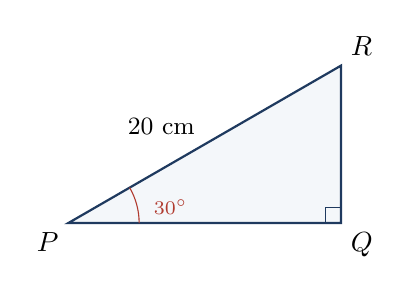
\begin{tikzpicture}
\coordinate (P) at (0,0); \coordinate (Q) at (3.464,0); \coordinate (R) at (3.464,2);
\draw[tri] (P)--(Q)--(R)--cycle;
\siku{P}{Q}{R}
\draw[brick] (0.9,0) arc (0:30:0.9); \node[brick,font=\scriptsize] at (1.3,0.2) {$30^\circ$};
\node[below left] at (P) {$P$}; \node[below right] at (Q) {$Q$}; \node[above right] at (R) {$R$};
\node[above left,font=\small,sloped] at (1.73,1) {$20$ cm};
\end{tikzpicture}}}{\hfill Jawaban: \rule{4.5cm}{0.4pt}}
\soal{Nilai dari $\dis\frac{\sin60^\circ\cdot\tan45^\circ+\cos30^\circ\cdot\csc30^\circ}{\sec60^\circ}$ adalah \dots}{\hfill Jawaban: \rule{4.5cm}{0.4pt}}
\soal{Jika $\tan\theta=2$ dengan $\theta$ sudut lancip, maka $\dis\frac{3\sin\theta-\cos\theta}{\sin\theta+\cos\theta}=$ \dots}{\hfill Jawaban: \rule{4.5cm}{0.4pt}}
\soal{\gbr{Dari puncak sebuah mercusuar setinggi $30$ m, seorang pengamat melihat sebuah kapal di laut dengan sudut depresi $30^\circ$. Jarak kapal ke kaki mercusuar adalah \dots\ m.}{%
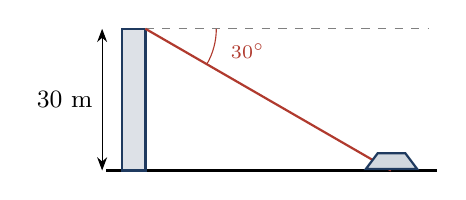
\begin{tikzpicture}
\draw[thick] (-0.5,0)--(3.7,0);
\fill[navy!15,draw=navy,thick] (-0.3,0) rectangle (0,1.8);
\draw[dashed,gray] (0,1.8)--(3.6,1.8);
\draw[thick,brick] (0,1.8)--(3.118,0);
\draw[brick] (0.9,1.8) arc (0:-30:0.9); \node[brick,font=\scriptsize] at (1.3,1.52) {$30^\circ$};
\draw[navy,thick,fill=navy!20] (2.8,0.02)--(3.45,0.02)--(3.3,0.22)--(2.95,0.22)--cycle;
\draw[<->,>=Stealth] (-0.55,0)--(-0.55,1.8); \node[left,font=\small] at (-0.55,0.9) {$30$ m};
\end{tikzpicture}}}{\hfill Jawaban: \rule{4.5cm}{0.4pt}}
\soal{Jika $\theta$ sudut lancip yang memenuhi $4\sin^{2}\theta-3=0$, maka $\tan\theta+\sec\theta=$ \dots}{\hfill Jawaban: \rule{4.5cm}{0.4pt}}

\bagian{C. Uraian (Essay)}{3 soal $\times$ 10 poin = 30 poin. Tuliskan langkah penyelesaian dengan lengkap.}
\soal{\gbr{Trapesium sama kaki $ABCD$ dengan $AB\parallel DC$, $AB=14$ cm, $DC=6$ cm, dan $AD=BC=8$ cm. Besar $\angle DAB=60^\circ$.\par\smallskip(a) Tentukan tinggi trapesium.\par(b) Tentukan luas trapesium.\par(c) Tentukan panjang diagonal $AC$.\par(d) Tentukan $\tan\angle CAB$.}{%
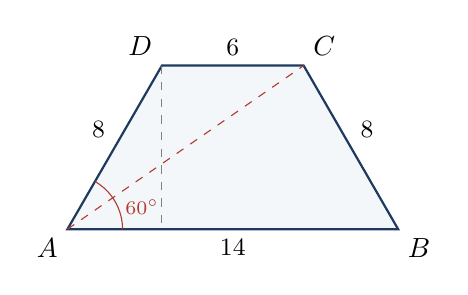
\begin{tikzpicture}
\coordinate (A) at (0,0); \coordinate (B) at (4.2,0); \coordinate (D) at (1.2,2.078); \coordinate (C) at (3.0,2.078);
\draw[tri] (A)--(B)--(C)--(D)--cycle;
\draw[dashed,brick] (A)--(C);
\draw[dashed,gray] (D)--(1.2,0);
\draw[brick] (0.7,0) arc (0:60:0.7); \node[brick,font=\scriptsize] at (0.95,0.28) {$60^\circ$};
\node[below left] at (A) {$A$}; \node[below right] at (B) {$B$}; \node[above right] at (C) {$C$}; \node[above left] at (D) {$D$};
\node[below,font=\small] at (2.1,0) {$14$}; \node[above,font=\small] at (2.1,2.078) {$6$};
\node[above left,font=\small] at (0.6,1.04) {$8$}; \node[above right,font=\small] at (3.6,1.04) {$8$};
\end{tikzpicture}}}{\poin{10}}
\soal{\gbr{Seorang pengamat berdiri di titik $P$ pada tanah datar, sejauh $30$ m dari kaki sebuah gedung. Di puncak gedung berdiri sebuah antena tegak lurus tanah. Dari $P$, puncak gedung terlihat dengan sudut elevasi $45^\circ$ dan puncak antena dengan sudut elevasi $60^\circ$ (abaikan tinggi pengamat).\par\smallskip(a) Tentukan tinggi gedung.\par(b) Tentukan tinggi puncak antena dari tanah.\par(c) Tentukan panjang antena (gunakan $\sqrt3\approx1{,}73$).\par(d) Tentukan jarak $P$ ke puncak antena.}{%
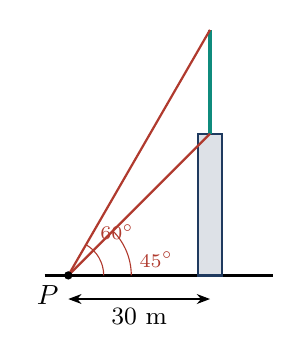
\begin{tikzpicture}
\draw[thick] (-0.3,0)--(2.6,0);
\fill[navy!15,draw=navy,thick] (1.65,0) rectangle (1.95,1.8);
\draw[ultra thick,teal] (1.8,1.8)--(1.8,3.118);
\draw[thick,brick] (0,0)--(1.8,1.8); \draw[thick,brick] (0,0)--(1.8,3.118);
\draw[brick] (0.8,0) arc (0:45:0.8); \node[brick,font=\scriptsize] at (1.12,0.2) {$45^\circ$};
\draw[brick] (0.45,0) arc (0:60:0.45); \node[brick,font=\scriptsize] at (0.62,0.55) {$60^\circ$};
\fill (0,0) circle (1.5pt); \node[below left] at (0,0) {$P$};
\draw[<->,>=Stealth] (0,-0.3)--(1.8,-0.3); \node[below,font=\small] at (0.9,-0.3) {$30$ m};
\end{tikzpicture}}}{\poin{10}}
\soal{(a) Dengan memakai segitiga siku-siku (sisi depan $d$, sisi samping $s$, sisi miring $m$), buktikan bahwa $\sin^{2}\theta+\cos^{2}\theta=1$ dan $1+\tan^{2}\theta=\sec^{2}\theta$.\par\smallskip(b) Jika $\theta$ sudut lancip dan $\sec\theta+\tan\theta=2$, tentukan $\sin\theta$.}{\poin{10}}

\newpage
\bagian{Kunci Jawaban dan Pembahasan Singkat}{Untuk guru dan pembahasan mandiri}
\par\vspace{0.6em}{\bfseries\color{navy}Kunci Pilihan Ganda}\par\vspace{0.3em}
\small
\begin{tabularx}{\linewidth}{@{}*{15}{>{\centering\arraybackslash}X}@{}}\hline \textbf{1} & \textbf{2} & \textbf{3} & \textbf{4} & \textbf{5} & \textbf{6} & \textbf{7} & \textbf{8} & \textbf{9} & \textbf{10} & \textbf{11} & \textbf{12} & \textbf{13} & \textbf{14} & \textbf{15}\\ \hline C & D & A & B & E & A & B & C & B & D & D & C & E & A & C\\ \hline\end{tabularx}
\par\vspace{0.8em}{\bfseries\color{navy}\normalsize Pembahasan Pilihan Ganda}\par\vspace{0.2em}
\small\begin{enumerate}[leftmargin=2em,itemsep=2pt,topsep=2pt]
\item[\textbf{1.}] \textbf{(C)} $PR=\sqrt{24^{2}+7^{2}}=25$. Sisi samping sudut $P$ adalah $PQ=24$, sehingga $\cos P=\dis\frac{24}{25}$.
\item[\textbf{2.}] \textbf{(D)} $\tan60^\circ\cos30^\circ=\sqrt3\cdot\dis\frac{\sqrt3}{2}=\dis\frac32$, lalu $\dis\frac32-\dis\frac12=1$.
\item[\textbf{3.}] \textbf{(A)} Samping $=15$, miring $=17$, depan $=\sqrt{17^{2}-15^{2}}=8$. Maka $\tan\theta=\dis\frac{8}{15}$.
\item[\textbf{4.}] \textbf{(B)} Dari tinggi mata ke puncak: $\tan45^\circ=\dis\frac{t'}{15}\Rightarrow t'=15$. Tinggi gedung $=15+1{,}5=16{,}5$ m (jangan lupa menambah tinggi mata).
\item[\textbf{5.}] \textbf{(E)} Depan $=3$, samping $=4$, miring $=5$. Maka $\sin\theta=\dis\frac35$ dan $\csc\theta=\dis\frac53$.
\item[\textbf{6.}] \textbf{(A)} $AC=10$. Karena $BD\perp AC$, $\angle DBC=90^\circ-\angle C=\angle A$. Jadi $\cos\angle DBC=\cos A=\dis\frac{AB}{AC}=\dis\frac{6}{10}=\dis\frac35$. (Cek: $BD=\dis\frac{6\cdot8}{10}=\dis\frac{24}{5}$, $\cos\angle DBC=\dis\frac{BD}{BC}=\dis\frac{24/5}{8}=\dis\frac35$.)
\item[\textbf{7.}] \textbf{(B)} Pembilang: $\left(\dis\frac12\right)^{2}+\left(\dis\frac{\sqrt2}{2}\right)^{2}=\dis\frac14+\dis\frac12=\dis\frac34$. Penyebut: $\sqrt3\cdot\sqrt3=3$. Hasilnya $\dis\frac34\div3=\dis\frac14$.
\item[\textbf{8.}] \textbf{(C)} $3\sin\theta=2\cos\theta\Rightarrow\tan\theta=\dis\frac23$. Depan $=2$, samping $=3$, miring $=\sqrt{13}$. Maka $\sin\theta\cos\theta=\dis\frac{2}{\sqrt{13}}\cdot\dis\frac{3}{\sqrt{13}}=\dis\frac{6}{13}$.
\item[\textbf{9.}] \textbf{(B)} Tinggi pada $60^\circ$: $8\sin60^\circ=4\sqrt3$. Tinggi pada $30^\circ$: $8\sin30^\circ=4$. Penurunan $=4\sqrt3-4=4\left(\sqrt3-1\right)$ m.
\item[\textbf{10.}] \textbf{(D)} Tinggi dari $A$ jatuh di tengah $BC$, sehingga setengah alas $=5$ dan tinggi $=\sqrt{13^{2}-5^{2}}=12$. Maka $\sin B=\dis\frac{12}{13}$, $\cos B=\dis\frac{5}{13}$, jumlahnya $\dis\frac{17}{13}$.
\item[\textbf{11.}] \textbf{(D)} Kuadratkan: $1+2\sin\theta\cos\theta=\dis\frac{49}{25}\Rightarrow\sin\theta\cos\theta=\dis\frac{12}{25}$. Maka $\tan\theta+\cot\theta=\dis\frac{\sin^{2}\theta+\cos^{2}\theta}{\sin\theta\cos\theta}=\dis\frac{1}{12/25}=\dis\frac{25}{12}$.
\item[\textbf{12.}] \textbf{(C)} Misal tinggi menara $h$ dan jarak $B$ ke kaki menara $x$. Dari $B$: $\tan60^\circ=\dis\frac hx\Rightarrow x=\dis\frac{h}{\sqrt3}$. Dari $A$: $\tan30^\circ=\dis\frac{h}{x+20}\Rightarrow x+20=h\sqrt3$. Kurangkan: $h\sqrt3-\dis\frac{h}{\sqrt3}=20\Rightarrow\dis\frac{2h}{\sqrt3}=20\Rightarrow h=10\sqrt3$ m.
\item[\textbf{13.}] \textbf{(E)} $BD=6\tan30^\circ=2\sqrt3$ dan $BC=6\tan60^\circ=6\sqrt3$, sehingga $DC=4\sqrt3$. Luas $ACD=\dis\frac12\cdot DC\cdot AB=\dis\frac12\cdot4\sqrt3\cdot6=12\sqrt3$ cm$^{2}$.
\item[\textbf{14.}] \textbf{(A)} $(\sin\theta-\cos\theta)^{2}=\dis\frac14\Rightarrow1-2\sin\theta\cos\theta=\dis\frac14\Rightarrow\sin\theta\cos\theta=\dis\frac38$. Maka $\sin^{4}\theta+\cos^{4}\theta=\left(\sin^{2}\theta+\cos^{2}\theta\right)^{2}-2\sin^{2}\theta\cos^{2}\theta=1-2\cdot\dis\frac{9}{64}=\dis\frac{23}{32}$.
\item[\textbf{15.}] \textbf{(C)} Sisi $a,\ ar,\ ar^{2}$ dengan $r>1$; sisi miring $ar^{2}$. Pythagoras: $a^{2}r^{4}=a^{2}+a^{2}r^{2}\Rightarrow r^{4}-r^{2}-1=0\Rightarrow r^{2}=\dis\frac{1+\sqrt5}{2}$. Sudut terkecil berhadapan dengan sisi $a$, maka $\sin=\dis\frac{a}{ar^{2}}=\dis\frac1{r^{2}}=\dis\frac{2}{1+\sqrt5}=\dis\frac{\sqrt5-1}{2}$.
\end{enumerate}
\par\Needspace{6\baselineskip}\vspace{0.6em}{\bfseries\color{navy}\normalsize Pembahasan Isian Singkat}\par\vspace{0.2em}
\small\begin{enumerate}[leftmargin=2em,itemsep=2pt,topsep=2pt]
\item[\textbf{1.}] \textbf{Jawaban: $\left(30+10\sqrt3\right)$ cm.} $QR$ di depan sudut $30^\circ$: $QR=20\sin30^\circ=10$. $PQ=20\cos30^\circ=10\sqrt3$. Keliling $=20+10+10\sqrt3=30+10\sqrt3$.
\item[\textbf{2.}] \textbf{Jawaban: $\dis\frac{3\sqrt3}{4}$.} $\sin60^\circ\tan45^\circ=\dis\frac{\sqrt3}{2}$ dan $\cos30^\circ\csc30^\circ=\dis\frac{\sqrt3}{2}\cdot2=\sqrt3$. Pembilang $=\dis\frac{3\sqrt3}{2}$, $\sec60^\circ=2$, sehingga hasilnya $\dis\frac{3\sqrt3}{4}$.
\item[\textbf{3.}] \textbf{Jawaban: $\dis\frac53$.} Bagi pembilang dan penyebut dengan $\cos\theta$: $\dis\frac{3\tan\theta-1}{\tan\theta+1}=\dis\frac{3\cdot2-1}{2+1}=\dis\frac53$.
\item[\textbf{4.}] \textbf{Jawaban: $30\sqrt3$ m.} Sudut depresi dari puncak sama dengan sudut elevasi dari kapal ($30^\circ$). $\tan30^\circ=\dis\frac{30}{d}\Rightarrow d=\dfrac{30}{1/\sqrt3}=30\sqrt3$ m.
\item[\textbf{5.}] \textbf{Jawaban: $2+\sqrt3$.} $\sin^{2}\theta=\dis\frac34\Rightarrow\sin\theta=\dis\frac{\sqrt3}{2}\Rightarrow\theta=60^\circ$. Maka $\tan60^\circ+\sec60^\circ=\sqrt3+2$.
\end{enumerate}
\par\Needspace{8\baselineskip}\vspace{0.6em}{\bfseries\color{navy}\normalsize Pembahasan dan Pedoman Penskoran Uraian}\par\vspace{0.2em}
\small\begin{enumerate}[leftmargin=2em,itemsep=3pt,topsep=2pt]
\item[\textbf{1.}] (a) Tinggi $=AD\sin60^\circ=8\cdot\dis\frac{\sqrt3}{2}=4\sqrt3$ cm. (b) Luas $=\dis\frac12(AB+DC)\cdot t=\dis\frac12(14+6)\cdot4\sqrt3=40\sqrt3$ cm$^{2}$. (c) Proyeksi $AD$ pada $AB$ adalah $8\cos60^\circ=4$, sehingga jarak mendatar $A$ ke $C$ adalah $4+6=10$. Maka $AC=\sqrt{10^{2}+(4\sqrt3)^{2}}=\sqrt{148}=2\sqrt{37}$ cm. (d) $\tan\angle CAB=\dis\frac{4\sqrt3}{10}=\dis\frac{2\sqrt3}{5}$. \\ \textit{Penskoran: (a) 3 poin; (b) 2 poin; (c) 3 poin; (d) 2 poin.}
\item[\textbf{2.}] (a) $\tan45^\circ=\dis\frac{t}{30}\Rightarrow t=30$ m. (b) $\tan60^\circ=\dis\frac{T}{30}\Rightarrow T=30\sqrt3\approx51{,}9$ m. (c) Panjang antena $=30\sqrt3-30=30\left(\sqrt3-1\right)\approx30(0{,}73)=21{,}9$ m. (d) $\cos60^\circ=\dis\frac{30}{PT}\Rightarrow PT=\dis\frac{30}{1/2}=60$ m. \\ \textit{Penskoran: (a) 3 poin; (b) 3 poin; (c) 2 poin; (d) 2 poin.}
\item[\textbf{3.}] (a) Pada segitiga siku-siku: $d^{2}+s^{2}=m^{2}$. Maka $\sin^{2}\theta+\cos^{2}\theta=\dis\frac{d^{2}}{m^{2}}+\dis\frac{s^{2}}{m^{2}}=\dis\frac{d^{2}+s^{2}}{m^{2}}=1$. Bagi kedua ruas dengan $\cos^{2}\theta$: $\tan^{2}\theta+1=\sec^{2}\theta$ (atau langsung: $1+\dis\frac{d^{2}}{s^{2}}=\dis\frac{s^{2}+d^{2}}{s^{2}}=\dis\frac{m^{2}}{s^{2}}$). (b) Dari $\sec^{2}\theta-\tan^{2}\theta=1$ diperoleh $(\sec\theta-\tan\theta)(\sec\theta+\tan\theta)=1$, sehingga $\sec\theta-\tan\theta=\dis\frac12$. Jumlahkan dan kurangkan dengan $\sec\theta+\tan\theta=2$: $\sec\theta=\dis\frac54$ dan $\tan\theta=\dis\frac34$. Maka $\cos\theta=\dis\frac45$ dan $\sin\theta=\tan\theta\cos\theta=\dis\frac35$. \\ \textit{Penskoran: bagian (a) 4 poin (masing-masing identitas 2 poin); bagian (b) 6 poin (hubungan $\sec-\tan$ 2 poin, nilai $\sec$ dan $\tan$ 2 poin, nilai $\sin\theta$ 2 poin).}
\end{enumerate}
\end{document}
